\graphicspath{{./figures/chapter4/}}
\lstset{inputpath = ../MATLAB}
\pgfplotstableset{search path = ./tables/chapter4}

\chapter{WENO reconstructions} \label{ch:WENO}

The reconstruction strategy based on least squares polynomial interpolation
that was introduced in Chapter \ref{ch:FVM} relies on a key technical assumption
about the exact solution $\vec{u}(\vec{x},t)$ of a hyperbolic system
of conservation laws: its smoothness in the neighborhood of every cell.
As we have seen in Section \ref{sec:conservation-laws}, however,
smooth solutions can develop discontinuities in finite time,
so it is necessary to investigate the behavior of these methods
when applied to discontinuous data, too.

On the one hand, the least squares system $\mat{V}_i \, \vec{p}_i = \bar{\vec{u}}$
is still well-defined even if the stencil $S_i$ of a cell $C_i$ crosses
a discontinuity, because the Vandermonde matrix $\mat{V}_i$ doesn't depend
on $\bar{\vec{u}}$. Hence, $\vec{p}_i$ can still be computed and evaluated
at $\vec{x}_{ijk}$ as before.

On the other hand, there is no guarantee that $\vec{p}_i(\vec{x}_{ijk})$
is an accurate approximation of $\vec{u}(\vec{x}_{ijk})$ anymore,
because error terms in a Taylor expansion of $\vec{u}$ don't hold
across a discontinuity. In the field of approximation theory, it is
well known that using the polynomial space $\Pi_K$ to approximate discontinuous
data is a bad idea, as undesired oscillations are produced in the neighborhood
of any discontinuity. This is exactly what happens when the methods
of the previous chapter are applied to the simulation of nonsmooth flows.

If the jumps in the cell averages $\bar{\vec{u}}_i$ are small enough,
LLS-$K$ methods can still produce quantitatively acceptable results,
despite their oscillatory behavior near the discontinuities.
For larger jumps, however, it may happen that $\vec{p}_i$ oscillates
so much that $\vec{p}_i(\vec{x}_{ijk}) \notin \mathcal{U}$, with $\mathcal{U}$
being the set of admissible values for a solution $\vec{u}(\vec{x},t)$
as defined at the end of Section \ref{sec:derivation-euler}.
For example, in the case of the compressible Euler equations, it may happen
that either the density or the pressure of a reconstruction on the border
of some cell becomes negative, and at that point there is no meaningful
way to continue the simulation.
This is exactly what happens when a LLS-$K$ reconstruction with $K \geq 2$
is used to solve the Riemann problem
\begin{equation} \label{eq:sod-shock-tube}
\vec{u}(x,y,0) = 
\begin{cases}
(1,0,0,(\gamma-1)^{-1}) &\text{if $x < 1/2$} \\
(1/8,0,0,(1/10)(\gamma-1)^{-1}) &\text{if $x \geq 1/2$} \\
\end{cases}
\end{equation}
for the 2D compressible Euler equations on the domain $[0,1] \times [0,1]$,
which is a standard test for the numerical solution of the compressible
Euler equations known as Sod's shock tube problem \cite{sod1978survey}.
The breakdown of the finite volume method was confirmed by a numerical
simulation; Programs \ref{prog:check-state2D} and \ref{prog:check-edges-state2D}
illustrate the MATLAB code that is used to check the admissibility
of the cell averages and of the reconstructions over the course of the simulation.

In the literature, numerous techniques have been developed to combine
high-order schemes with nonoscillatory behavior near discontinuities.
Among them, one of the most popular, versatile and effective technique
is Weighted Essentially NonOscillatory (WENO) approximation,
first introduced for one-dimensional problems by Liu, Osher and Chan in 1994 as an
improvement over earlier ENO interpolation \cite{liu1994weighted}.
Later, WENO reconstructions were generalized to 2D problems on triangular
meshes by Hu and Shu \cite{hu1999weighted}.
For an introduction to WENO schemes and all of its possible
applications in the field of approximation theory, we refer
to the very accessible review article by Shu \cite{shu2009high}.
For the classical theory of WENO schemes on tensor product grids,
we refer to Shu's lecture notes \cite{cockburn2006advanced}
and to Chapter 11 of the recent book by Hestaven \cite{hesthaven2017numerical}.

The main idea behind WENO reconstructions is to choose multiple
interpolation stencils $S_{i\ell}$ on every cell $C_i$, so that different
least squares polynomial reconstructions $\vec{p}_{i\ell}(\vec{x})$ are defined,
and then to take as an approximation of $\vec{u}(\vec{x},t)$ on $\partial C_i$
a convex combination
\begin{equation} \label{eq:WENO-convex-combination}
\vec{p}_i = \sum_{\ell} \omega_{i\ell} \, \vec{p}_{i\ell}
\end{equation}
of all polynomials $\vec{p}_{i\ell}$, each one weighted by a coefficient
$\omega_{i\ell}$ that depends on a \emph{smoothness indicator}
$S\!I(\vec{p}_{i\ell})$ (a better name would be \emph{oscillation functional},
but this is how it is known in the literature).
In this way, oscillatory reconstructions are penalized, and all that is needed
to get an essentially nonoscillatory reconstruction is to have at least one
nonoscillatory polynomial~$\vec{p}_{i\bar{\ell}}$ in the convex combination
\eqref{eq:WENO-convex-combination}.
To achieve this, one-sided stencils that span different directions are used
in addition to a centered stencil like that of Chapter \ref{ch:FVM}:
if the strategy is successful, at least one of the stencils will not cross
a discontinuity and will therefore produce the required nonoscillatory
polynomial~$\vec{p}_{i\bar{\ell}}$.
Since the weights $\omega_{i\ell}$ depend nonlinearly on $\vec{p}_{i\ell}$,
and hence nonlinearly on $\bar{\vec{u}}_i(t)$, WENO schemes are
said to be \emph{nonlinear schemes}, unlike the LLS-$K$ schemes
of Chapter \ref{ch:FVM}.

In \cite{liu2013robust}, Liu and Zhang introduced the distinction
between type-I and type-II WENO interpolations.
The first type consists of WENO reconstructions whose order of accuracy is
not higher than that of the reconstruction on each stencil.
For this type of WENO reconstruction, the nonlinear weights do not
contribute towards the increase of the order of accuracy, because they are
designed purely for the purpose of nonlinear stability and to avoid
spurious oscillations in the numerical solution.
We remark that a convex combination like \eqref{eq:WENO-convex-combination}
of $K$-exact reconstructions $\vec{p}_{i\ell}$ is itself a $K$-exact
reconstruction, so type-I WENO schemes have order $K$ if the
exact solution $\vec{u}(\vec{x},t)$ is sufficiently smooth.

The second type consists of WENO reconstructions whose order of accuracy in regions
where $\vec{u}(\vec{x},t)$ is smooth is higher than that of the reconstruction
on each stencil, typically by a factor of 1.
For example, a third order type-II WENO interpolation on a 2D mesh can be
based on second order linear polynomial reconstructions on each stencil.
For this type of WENO reconstruction, the nonlinear weights contribute
towards the increase of the order of accuracy, because the overall
reconstruction is given at each quadrature node $\vec{x}_{ijk}$ by a weighted
average of the lower order reconstructions (in this case, the weights
$\omega_{i\ell}$ must depend on the indices $j$ and $k$ in addition to $i$ and $\ell$).

In the next section we propose a generalization of type-I WENO reconstructions
to arbitrary polygonal meshes. This is something that, to the best of our
knowledge, has never been tried before; our first results are encouraging.

\section{Type-I WENO reconstructions on polygonal meshes}
Suppose that on each cell $C_i$ a collection
$\{S_{i\ell}\}_{\ell = 1 \dots N_S(i)}$ of $N_S(i)$ distinct stencils
has been defined, and let $m_{i\ell}$ be the size of each stencil $S_{i\ell}$.
Let $\vec{p}_{i\ell}$ be the polynomial of degree $K$ obtained by
the least squares procedure of Chapter \ref{ch:FVM} from the cell averages
$\{\bar{\vec{u}}_\kappa \mid \kappa \in S_{i\ell}\}$.
Then, we define our type-I WENO reconstruction by the convex combination
\begin{equation} \label{eq:WENO}
\vec{p}_i = \sum_{\ell} \omega_{i\ell} \, \vec{p}_{i\ell},
\end{equation}
which is evaluated on every quadrature node $\vec{x}_{ijk}$ of cell $C_i$
to produce either $\vec{u}_{ijk}^+$ or $\vec{u}_{ijk}^-$, depending on whether
the normal $\vec{\nu}_{ij}$ points into $C_i$ or away from $C_i$, respectively.
The weights $\omega_{i\ell}$ are obtained by normalizing another set
of strictly positive weights $\tilde{\omega}_{i\ell}$:
\[
\omega_{i\ell} = \frac{\tilde{\omega}_{i\ell}}
                      {\sum_{\ell=1}^{N_S(i)} \tilde{\omega}_{i\ell}}.
\]
It is these weights $\tilde{\omega}_{i\ell}$ that, as anticipated,
depend on the smoothness indicator $S\!I(\vec{p})$. This indicator should give
us an estimate of how strongly a polynomial $\vec{p}$ oscillates on $C_i$;
a standard choice for $S\!I(\vec{p})$ is to define it as the sum of the squares
of the $L^2$ norms of all the derivatives of $\vec{p}$ of order 1 to $K$:
\[
S\!I(\vec{p}) \deq \sum_{1 \leq \abs{\alpha} \leq K} \frac{1}{\abs{C_i}}
	\int_{C_i} h_i^{2\abs{\alpha}} \bigl(\partial_\alpha \vec{p}(x,y)\bigr)^2 \dxy
\]
The sum is taken over a two-dimensional multi-index $\alpha$.
The terms $\abs{C_i}^{-1}\!$ and $h_i^{2\abs{\alpha}}$ are introduced
to make the smoothness indicator scale-invariant with respect to the
size of $C_i$.
% Under the assumption of shape regularity
%(see Definition \ref{defi:shape-regularity}),
This can be proved by switching to the same local coordinates $(\xi,\eta)$
that were used in Chapter \ref{ch:FVM} to keep the condition number
of the least squares system bounded as $h \to 0$.
%\[
%(\xi,\eta) \deq \left( \frac{x-x_i}{h_i}, \frac{y-y_i}{h_i} \right)
%\qquad \varphi(x,y) \deq \left( \frac{x-x_i}{h_i}, \frac{y-y_i}{h_i} \right)
%\quad \varphi \colon C_i \to \hat{C}_i
%\]
%with $(x_i,y_i)$ barycenter of cell $C_i$.

As in every WENO scheme, the unnormalized weights $\tilde{\omega}_{i\ell}$
are then defined by
\begin{equation} \label{eq:unnormalized-weights}
\tilde{\omega}_{i\ell} = \frac{c_\ell}{(\varepsilon + S\!I(\vec{p}_{i\ell}))^r}
\qquad \varepsilon,r > 0.
\end{equation}
We now see why oscillating reconstructions are penalized: for any
polynomial $\vec{p}_{i\ell}$, a larger value of the functional
$S\!I(\vec{p}_{i\ell})$ corresponds to a smaller unnormalized weight
$\tilde{\omega}_{i\ell}$.
The coefficients $c_\ell > 0$ are known as \emph{linear coefficients} of the
reconstruction, and if dependent on $j$ and $k$ provide type-II WENO
schemes the necessary degrees of freedom to achieve higher orders of convergence.
Since we are only dealing with type-I WENO reconstructions in this work,
we can simply take $c_\ell = 1$ for all $\ell = 1, \dots, N_S(i)$,
on the principle that equally oscillating polynomials should
get the same weights in formula \eqref{eq:WENO}.

The parameters $\varepsilon$ and $r$ in \eqref{eq:unnormalized-weights}
can be tuned depending on the problem that has to be solved.
The parameter $\varepsilon$ is a small positive number used to avoid division by zero.
$S\!I(\vec{p}_{i\ell}) = 0$ if and only if $\vec{p}_{i\ell}$ is a constant
polynomial, so smaller values of $\varepsilon$ emphasize the fact
that constant reconstructions are assigned larger weights compared
to nonconstant ones.
The positive exponent $r$ controls the sensitivity of the unnormalized weights
with respect to the oscillation indicator. When $r \to \infty$, the reconstruction
$\vec{p}_i$ converges to the least oscillating polynomial among
$\{\vec{p}_{i\ell}\}_{\ell = 1 \dots N_S(i)}$,
whereas for $r \to 0$ the reconstruction $\vec{p}_i$ converges to the
arithmetic mean of all the polynomials $\{\vec{p}_{i\ell}\}_{\ell = 1 \dots N_S(i)}$.
In practice, the choices $\varepsilon = 10^{-6}$ and $r = 4$ give satisfactory
results for most problems.

\subsection*{Choice of stencils}
As we have already pointed out in the introduction to this chapter,
WENO reconstructions are nonoscillatory only if at least one of the
stencils $S_{i\ell}$ does not cross a discontinuity.
Therefore, it makes sense in this context to consider stencils
that look like circular sectors rather than circles: in this way,
even if a cell $C_i$ is right next to a shock, we can find a stencil
that points in the opposite direction of the shock, and that stencil
should give us the nonoscillatory reconstruction that we are looking for.

To make this idea mathematically precise, let us denote the barycenter
of each cell $C_i$ with $\vec{x}_i$, and let
$A(\vec{x}_i,\vec{x}_\ell,\vec{x}_\kappa)$ be the angle in $\R^2$
formed by the left and right rays
\[
\{ \vec{x}_i + \tau (\vec{x}_\ell - \vec{x}_i) \mid \tau \geq 0 \},
\qquad
\{ \vec{x}_i + \tau (\vec{x}_\kappa - \vec{x}_i) \mid \tau \geq 0 \}.
\]
Then, for each cell $C_i$ and for each pair $C_\mu, C_\lambda$
of adjacent cells in consecutive counterclockwise order with respect
to $C_i$, we would like to define a one-sided stencil $S_{i\ell}$
that covers a region of $\R^2$ with a shape that resembles
$A(\vec{x}_i,\vec{x}_\lambda,\vec{x}_\mu)$ as much as possible.
The idea is to once again consider the adjacency graph $G$ of the given
tessellation $\mathcal{T}_h$ and define the set
\[
D_A(C_i,r) = \{ C_\ell
	\mid d(C_i,C_\ell) \leq r \text{ and } C_\ell \cap A \neq \emptyset\}
\]
as the collection of all cells in $\mathcal{T}_h$ that have graph distance
at most $r$ from $C_i$ and that touch a given angle $A$. Let $n_i$ be the
dimension of the polynomial space $\Pi_K$. Then, for each pair $C_\mu, C_\lambda$
of adjacent cells in consecutive counterclockwise order with respect
to $C_i$, our heuristic is to define $S_{i\ell}$ as the set
$D_{A(\vec{x}_i,\vec{x}_\lambda,\vec{x}_\mu)}(C_i,\bar{r})$,
with $\bar{r} \in \N$ being the smallest non-negative integer such that
$D_{A(\vec{x}_i,\vec{x}_\lambda,\vec{x}_\mu)}(C_i,\bar{r})$ has at least
$n_i$ elements.

\begin{figure}[tbp]
\centering
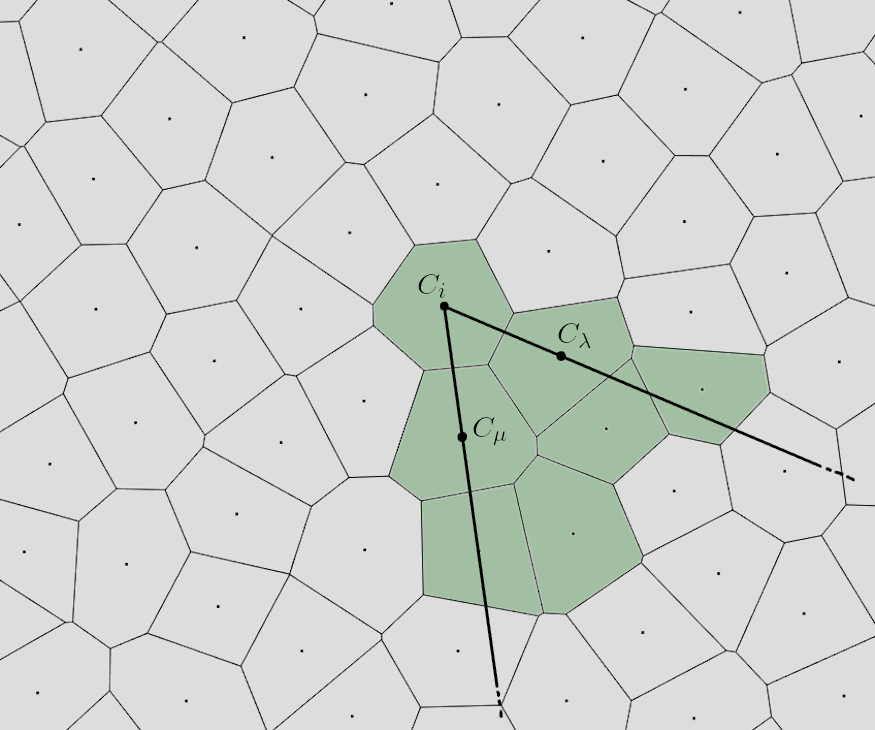
\includegraphics[width=0.48\textwidth]{cellsWENO1.png}
\hfill
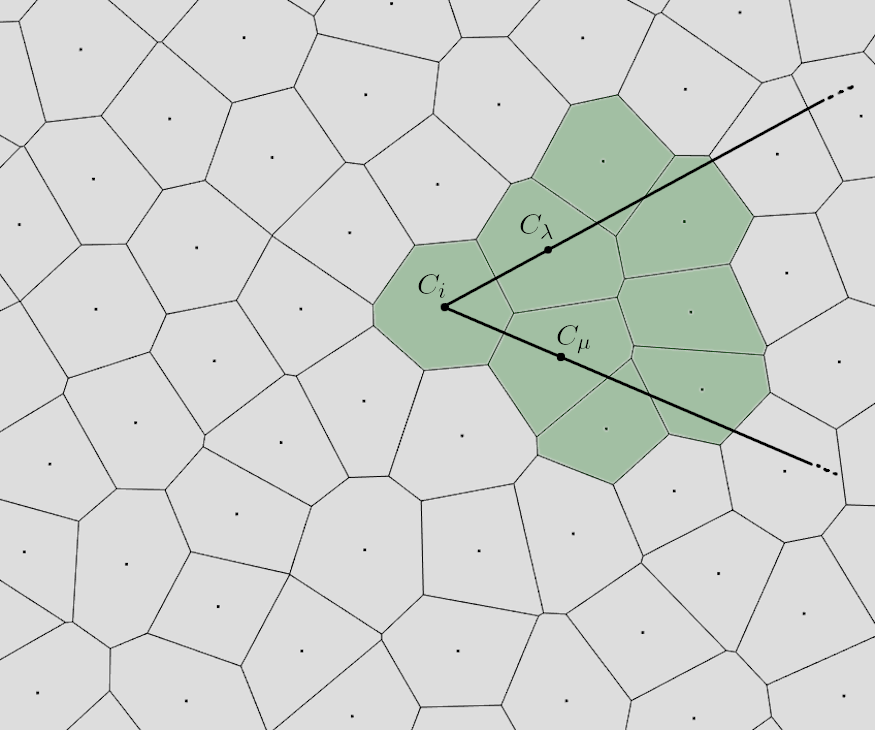
\includegraphics[width=0.48\textwidth]{cellsWENO2.png}
\caption{Examples of one-sided stencils for quadratic WENO reconstructions.}
\label{fig:stencils}
\end{figure}

\subsection*{Implementation details}
Once again, the stencils $S_{i\ell}$ can be efficiently computed
by a breadth-first search algorithm on the graph $G$ with starting node
$C_i$ and with the angle $A(\vec{x}_i,\vec{x}_\lambda,\vec{x}_\mu)$
working as a kind of filter on the cells, as implemented in the
\code{C++} function \code{build\_onesided\_stencil()} contained in
Program \ref{prog:reconstruction}.
Figure \ref{fig:stencils} shows some typical outputs of this algorithm.
Green cells belong to the one-sided stencils, while gray cells do not;
the barycenters $\vec{x}_i, \vec{x}_\lambda, \vec{x}_\mu$ are highlighted.

WENO reconstructions of order $K$ up to 3 are implemented in
Program \ref{prog:reconstruction-T1WENO}. The condition number
of $\mat{V}_{i\ell}$, even if bounded by switching to local coordinates
$(\xi,\eta)$, could be much higher for a one-sided stencil compared to
a centered stencil. Therefore, while solving the least squares problem
in function \code{least\_squares\_and\_condition\_number} of Program
\ref{prog:reconstruction} we use the LAPACK routine \code{DTRCON}
on the upper-triangular factor R of the QR decomposition
of $\mat{V}_{i\ell}$: in this way, we get almost for free an estimate
on the condition number of $\mat{V}_{i\ell}$ and, if it is above
a certain threshold, we remove the polynomial $\vec{p}_{i\ell}$ from
the convex combination \eqref{eq:WENO-convex-combination}.
Just to make sure that we do not discard all stencils, we always include
in \eqref{eq:WENO-convex-combination} the polynomial reconstruction
given by a centered stencil (the same as in LLS-$K$ schemes).

The numerical treatment of boundary conditions that we have
seen in Section \ref{sec:boundary-condtions} is also adequate
for WENO schemes; the only difference is that, for added robustness
when a planar shock wave hits a wall, we progressively reduce the order
of the WENO scheme next to the boundary of the domain.

\section{Numerical tests in the nonsmooth case}

\subsection*{Sod's shock tube problem}
As a first test, we solve Sod's shock tube problem
\eqref{eq:sod-shock-tube} using WENO reconstructions of increasing order.
The domain $\Omega = [0,1] \times [0,1]$ is discretized with
a 512$\times$512 square grid. Since the Riemann problem
described by \eqref{eq:sod-shock-tube} is essentially
a 2D extension of a 1D problem, we put periodic boundary conditions
on the top and bottom sides of $\partial\Omega$.
As for the left and right sides, we choose wall boundary conditions,
although this is not really important because we stop the
simulation before any of the perturbations in the fluid can reach
the end of the tube.
If $K = 1$ or $K = 2$, we put one quadrature point on each edge, else two.
An SSPRK method of order $K$ is used for the numerical solution
of the system of ordinary differential equations produced by the
finite volume method. As for WENO parameters, we choose
$\varepsilon = 10^{-12}$ and $r = 4$. Such a small $\varepsilon$
is well-suited for Riemann problems like \eqref{eq:sod-shock-tube},
because we expect large regions of the solution to be constant.

Figure \ref{fig:sod} shows the density of the numerical solution
at time $T = 0.2$ as a function of~$x$ (both the continuous and the discrete
solutions are constant with respect to $y$). The exact solution contains
a rarefaction wave between $x \approx 0.263$ and $x \approx 0.486$,
a contact discontinuity at $x \approx 0.685$, and a shock wave at $x \approx 0.85$.
Figure \ref{fig:sod-closeup} zooms in on the most interesting
parts of the previous figure. We can clearly see that higher order
WENO methods have sharper transitions around discontinuities,
especially the contact discontinuity, but are nevertheless nonoscillatory.
This is exactly the behavior that we hoped to achieve by introducing
WENO reconstructions.

\begin{figure}[p]
\centering
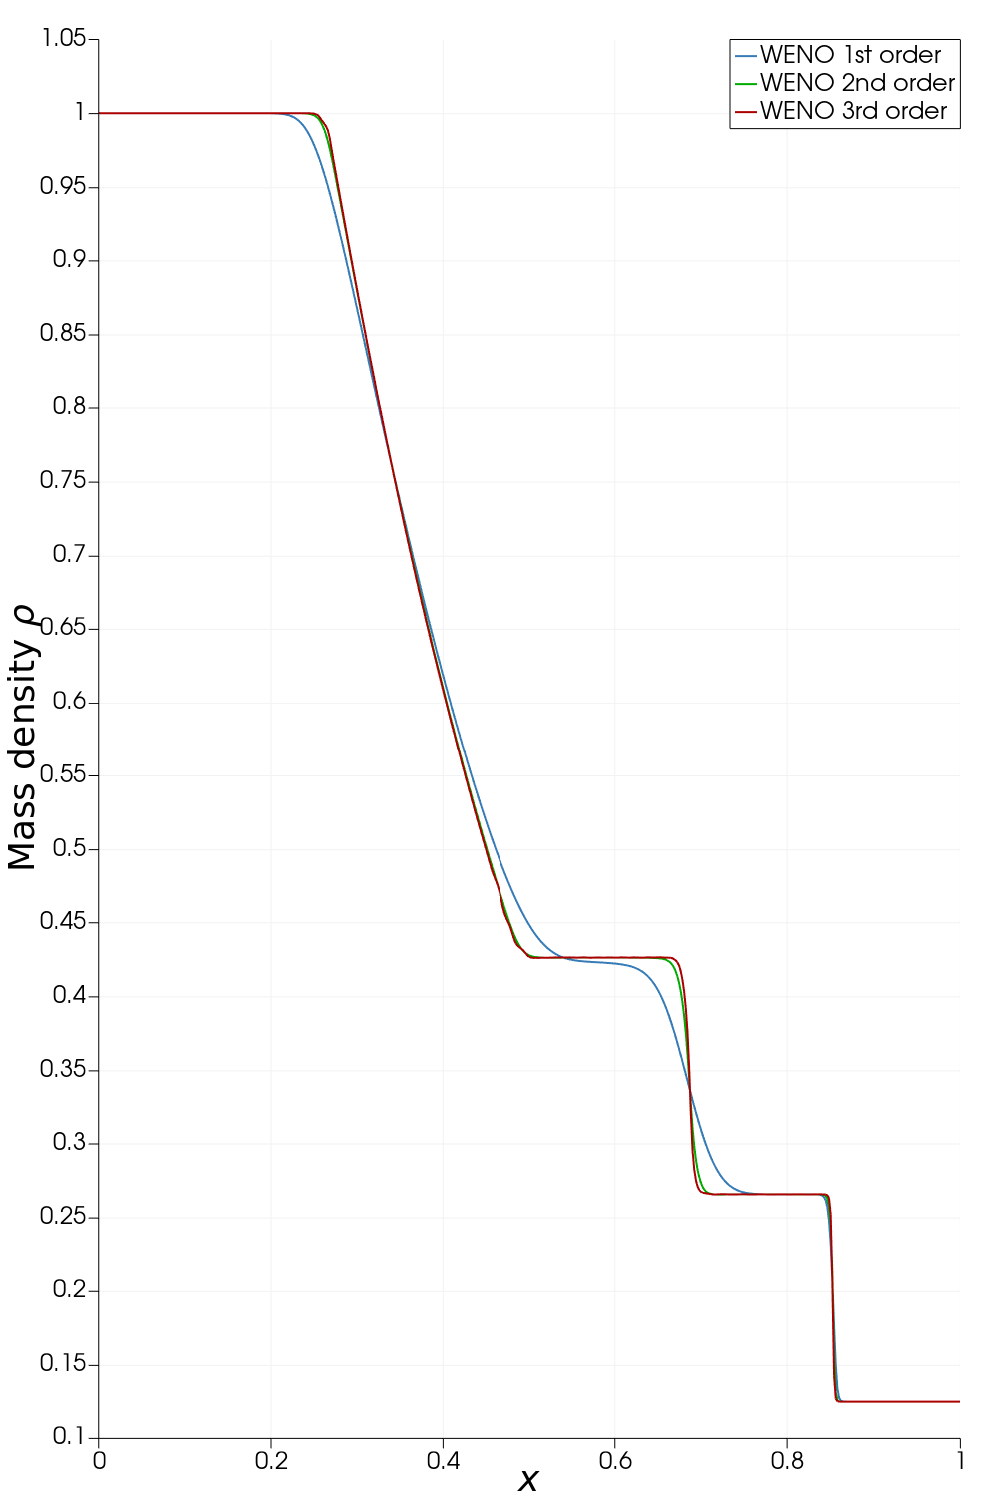
\includegraphics[width=0.98\textwidth]{sod1.png}
\caption{Numerical solution of Sod's shock tube problem at $t = 0.2$.}
\label{fig:sod}
\end{figure}

\begin{figure}[p]
\centering
\subcaptionbox{Left end of the rarefaction wave.} {
	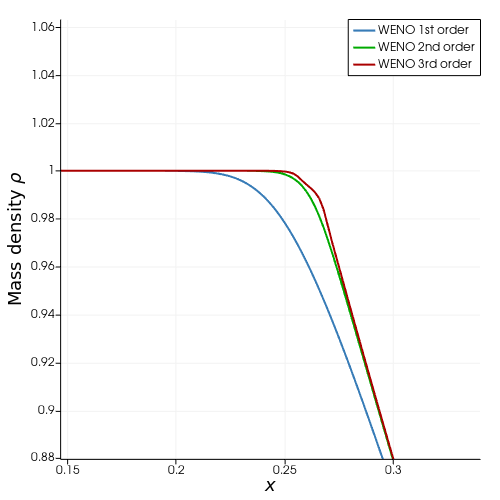
\includegraphics[width=0.47\textwidth]{sod2.png}
} \hfill
\subcaptionbox{Right end of the rarefaction wave.} {
	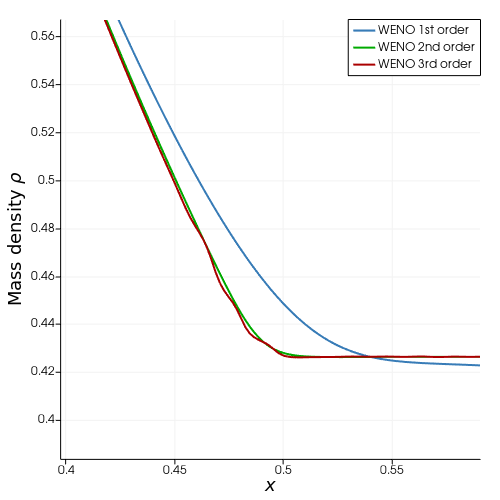
\includegraphics[width=0.47\textwidth]{sod3.png}
} \\[2em]
\subcaptionbox{Contact discontinuity.} {
	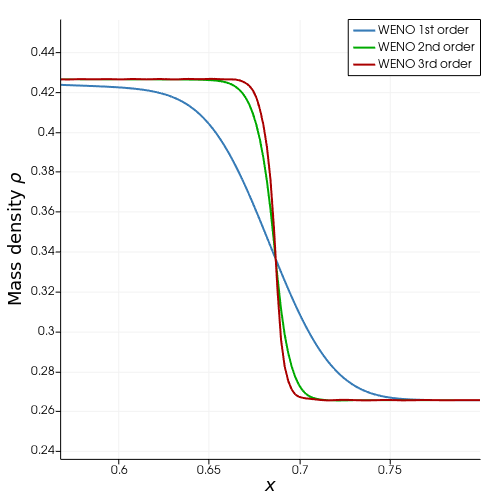
\includegraphics[width=0.47\textwidth]{sod4.png}
} \hfill
\subcaptionbox{Shock wave.} {
	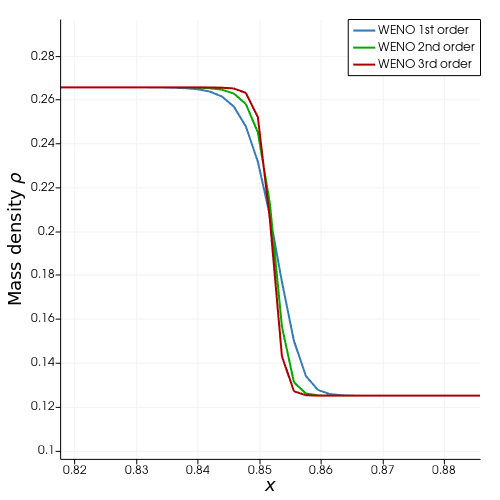
\includegraphics[width=0.47\textwidth]{sod5.png}
}
\caption{Details of the numerical solution of Sod's shock tube problem at $t = 0.2$.}
\label{fig:sod-closeup}
\end{figure}

\subsection*{Elliptical whispering gallery}
Consider an elliptical domain $\Omega$ whose border is defined implicitly
by the equation
\[
\frac{x^2}{a^2} + \frac{y^2}{b^2} = 1,
\]
with semi-major axis $a > 0$ and semi-minor axis $b \in (0,a)$.
Then, the foci $\vec{F}_1, \vec{F}_2$ of the ellipse have coordinates
\[
\vec{F}_1 = (-\sqrt{a^2 - b^2}, 0), \quad \vec{F}_2 = (\sqrt{a^2 - b^2}, 0)
\]
and it is possible to prove that $\partial \Omega$ is the locus
of points $\vec{x}$ in the Euclidean plane such that the sum of the distances
$\norm{\vec{x}-\vec{F}_1}$ and $\norm{\vec{x}-\vec{F}_2}$ is equal to $2a$:
\[
\partial\Omega = \{ \vec{x} \in \R^2 \mid
\norm{\vec{x}-\vec{F}_1} + \norm{\vec{x}-\vec{F}_2} = 2a \}.
\]
An interesting geometrical property of an ellipse is that, for each point
$\vec{x} \in \partial\Omega$, the normal $\vec{\nu}(\vec{x})$ to the
border is a bisector of the angle formed by the rays
\[
\{ \vec{x} + \tau (\vec{F}_1 - \vec{x}) \mid \tau \geq 0 \},
\qquad
\{ \vec{x} + \tau (\vec{F}_2 - \vec{x}) \mid \tau \geq 0 \}.
\]
This in turn implies that the reflection on $\partial\Omega$ of any ray
originating from one of the foci necessarily passes through the other
focus after having traveled a distance $2a$.
An acoustic consequence of this property is that, in an elliptical room
under ideal conditions, a whisper by a person standing at $\vec{F}_1$
will be heard by another person standing at $\vec{F}_2$ regardless
of the distance $2a$: elliptical rooms make excellent whispering galleries.

In this second numerical test, our aim is to reproduce this acoustic
phenomenon using a finite volume scheme based on WENO reconstructions
of order two. For this purpose, we fix an elliptical domain $\Omega$
and simulate the time evolution of a very narrow Gaussian perturbation on
the initial pressure and density fields localized at $\vec{F}_1$.
Let $A$ be the amplitude and $\sigma$ be the width of the Gaussian perturbation.
Then, we consider the following initial conditions for $\vec{u}$, here
expressed in the more convenient variables $(\rho,\vec{v},p)$:
\begin{equation} \label{eq:ellipse-initial-conditions}
\begin{gathered}
\vec{u}_0(\vec{x}) =
\begin{pmatrix}
\rho_\infty  \bigl( 1 + A \exp(-\norm{\vec{x}-\vec{F}_1}/(2\sigma^2) \bigr) \\ 
\vec{v}_\infty \\
p_\infty \bigl( 1 + A \exp(-\norm{\vec{x}-\vec{F}_1}/(2\sigma^2) \bigr)
\end{pmatrix} \\
\rho_\infty = \SI{1,225}{\kg\per\meter\cubed},
\quad \vec{v}_\infty = 0,
\quad p_\infty = \SI{101325}{\pascal},
\quad A = 0.1,
\quad \sigma = 0.2
\end{gathered}
\end{equation}
%The freestream values $(\rho_\infty,\vec{v}_\infty,p_\infty)$ are
The initial condition is smooth, but also very steep in a neighborhood
of $\vec{F}_1$. Since a numerical scheme can hardly distinguish
between discontinuities and very strong gradients in the data,
WENO schemes are required to prevent spurious oscillations
near the wave fronts.
The size of the ellipse $\Omega$ is defined using a Pythagorean triple, so that
\[
a = 29, \quad b = 21, \quad \vec{F}_1 = (-20,0), \quad \vec{F}_2 = (20,0),
\]
and $\Omega$ is discretized by the Voronoi technique explained in
Section \ref{sec:mesh-generation}. Figure \ref{fig:ellipse-2500} shows what a
tessellation of $\Omega$ looks like with $N_c = 1415$; for our simulation we choose
a much finer partition with $N_c = 21599$. Wall boundary conditions
are chosen on the entirety of $\partial\Omega$. Since $K = 2$, a single
quadrature point on each edge will suffice. An SSPRK method of order $2$
is used for the numerical solution of the system of ordinary differential
equations produced by the finite volume method. As for WENO parameters,
we choose $\varepsilon = 10^{-8}$ and $r = 4$.
The speed of sound in the unperturbed fluid is
\[
c_\infty = \sqrt{\frac{\gamma p_\infty}{\rho_\infty}}
\approx \SI{340,3}{\meter\per\second},
\]
therefore we expect the sound waves caused by the perturbation
of the initial data to reach $\vec{F}_2$ after approximately
$t_f \deq 2a/c_\infty \approx \SI{0.17}{\second}$.
Indeed, looking at the results in Figure \ref{fig:ellipse-simulation}
we can see that, after an initial dispersion of the Gaussian perturbation,
the acoustic waves reflect on the walls as expected and eventually
reach $\vec{F}_2$.
Of course, numerical diffusion prevents the spike in pressure
at $\vec{F}_2$ to be as high and localized as it was in the initial
conditions, but it is still significantly higher than every single
wave front at time $t_f/2$, meaning that a simultaneous superposition
of waves was achieved. Figure \ref{fig:ellipse-F2} confirms that the spike
in pressure is exactly at $\vec{x} = (20,0)$, as expected.

The significance of this test is manifold. First of all, the correct
treatment of the wall boundary conditions is checked, since waves
are able to correctly reflect off the walls at every possible angle
of incidence.
Second, the test confirms that waves are traveling at the correct speed,
since they all reach $\vec{F}_2$ at the same time.
Third, the values of pressure are nonoscillatory. Figure
\ref{fig:ellipse-P001} shows a section of the numerical solution
on the horizontal line $y = 0$ at time $t = 0.01$,
and the transition from the wave fronts to the unperturbed fluid
are indeed monotone.
The bump in pressure at $\vec{F}_1$ is not a numerical artifact,
but an actual feature of the exact solution.

\begin{figure}[tbp]
\centering
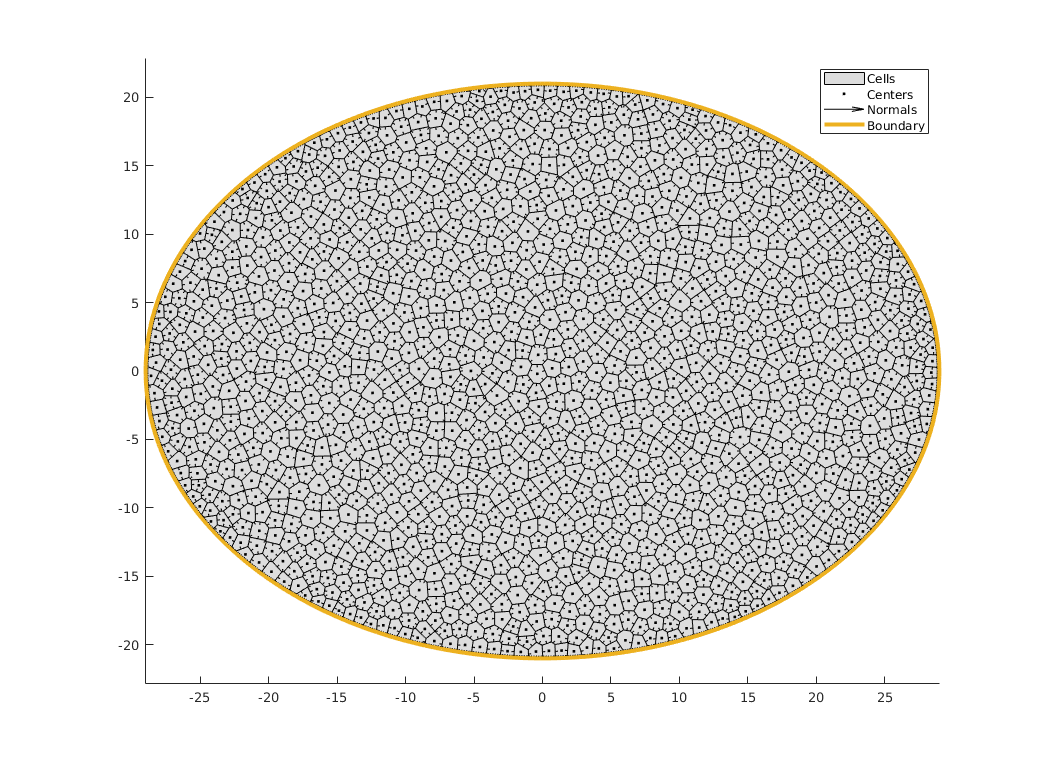
\includegraphics[width=0.8\textwidth]{ellipse2500.png}
\caption{Polygonal discretization of the ellipse, 1415 Voronoi cells.}
\label{fig:ellipse-2500}
\end{figure}

\clearpage

\begin{figure}[p]
\centering
\subcaptionbox{Pressure at $t = 0$} {
	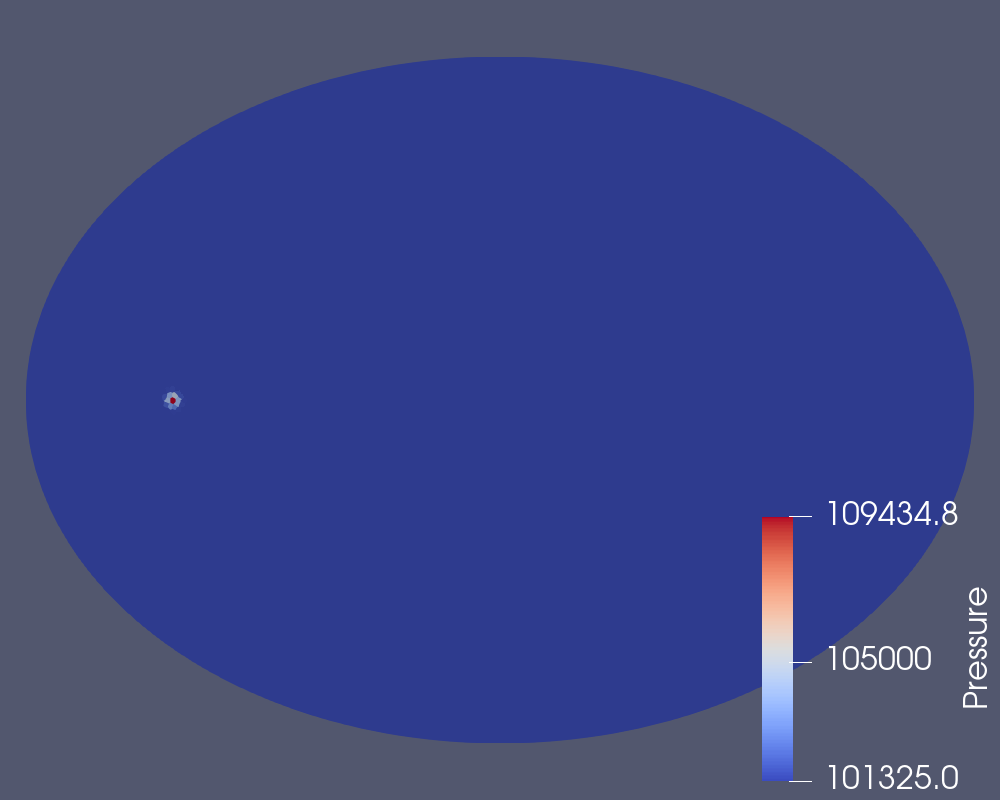
\includegraphics[width=0.47\textwidth]{ellipset0.png}
} \hfill
\subcaptionbox{Pressure at $t = 0.01$} {
	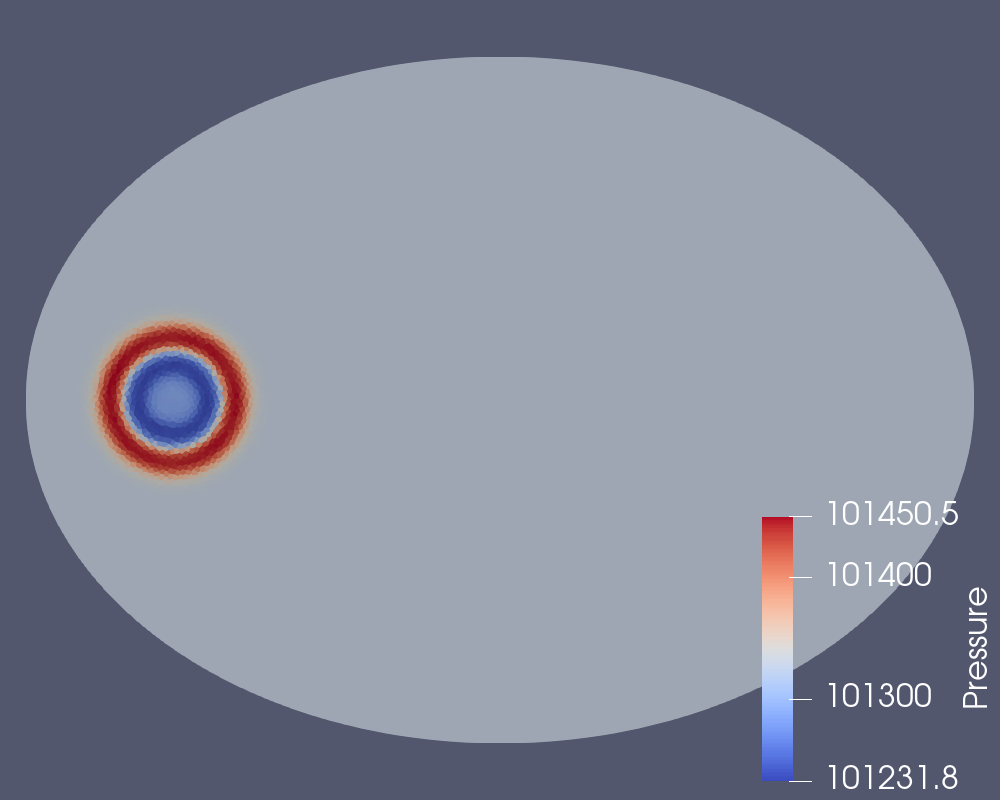
\includegraphics[width=0.47\textwidth]{ellipset001.png}
} \\[2em]
\subcaptionbox{Pressure at $t = 0.05$} {
	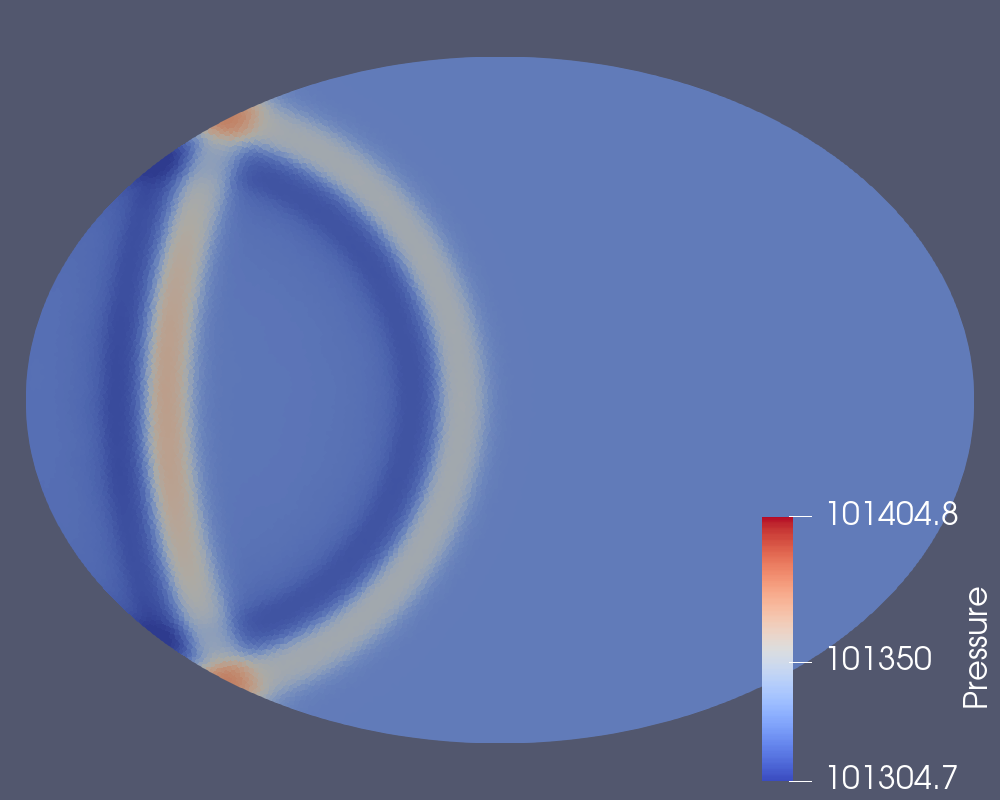
\includegraphics[width=0.47\textwidth]{ellipset005.png}
} \hfill
\subcaptionbox{Pressure at $t = 0.1$} {
	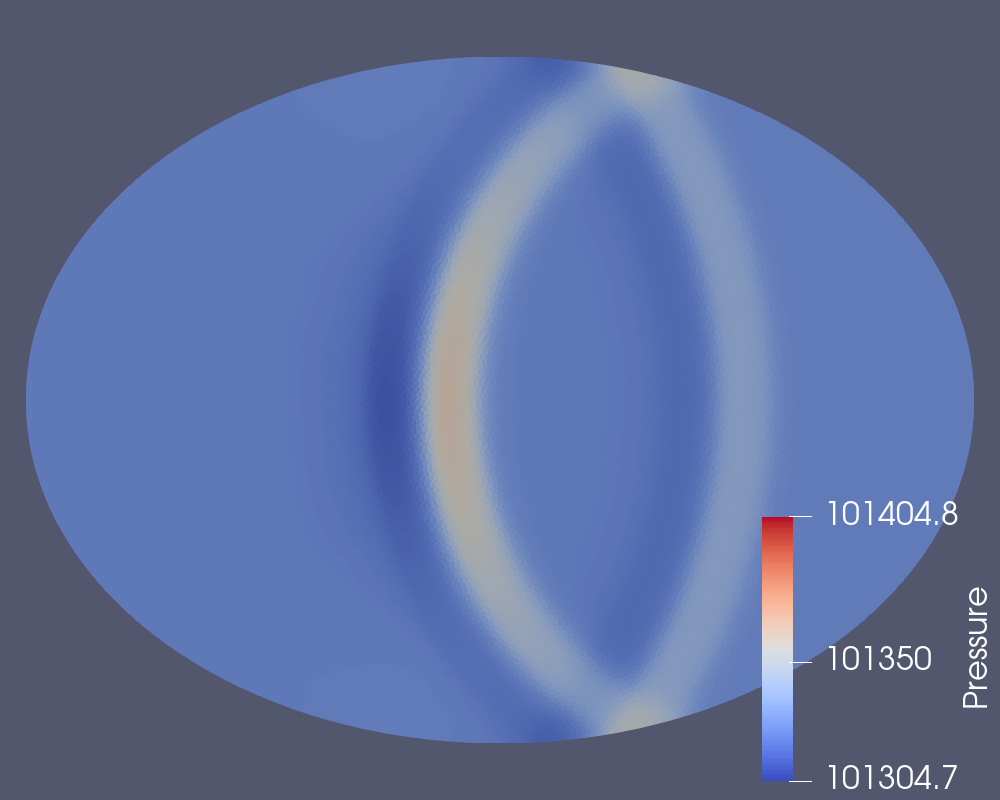
\includegraphics[width=0.47\textwidth]{ellipset010.png}
} \\[2em]
\subcaptionbox{Pressure at $t = 0.15$} {
	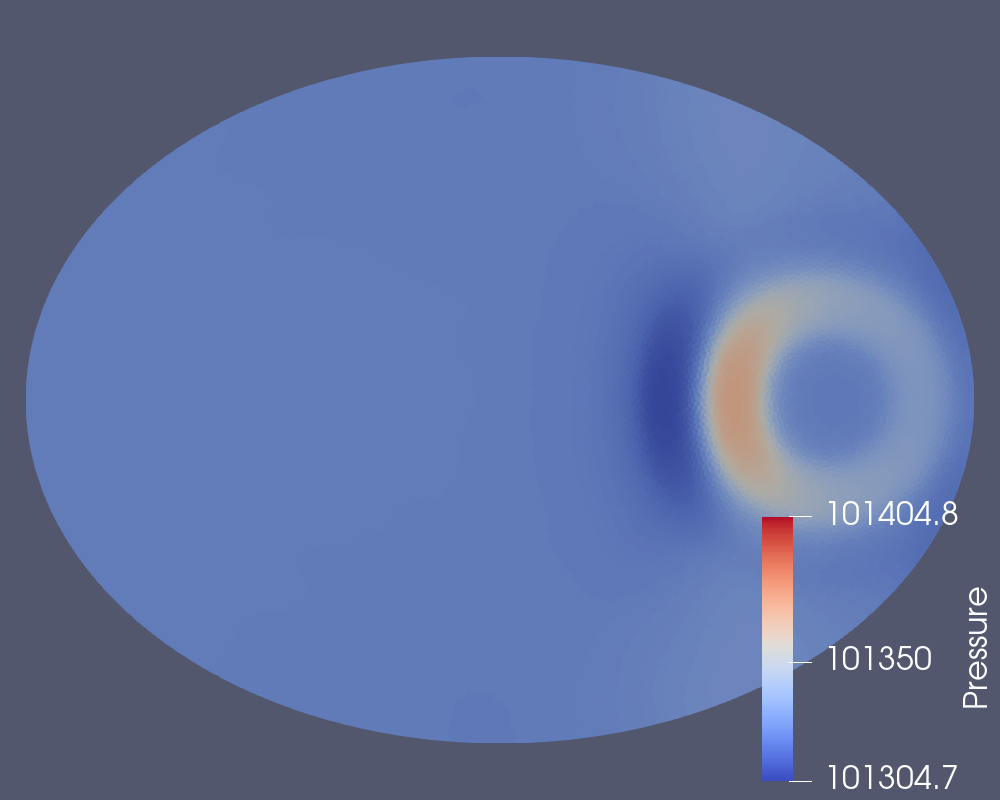
\includegraphics[width=0.47\textwidth]{ellipset015.png}
} \hfill
\subcaptionbox{Pressure at $t = 0.1645$} {
	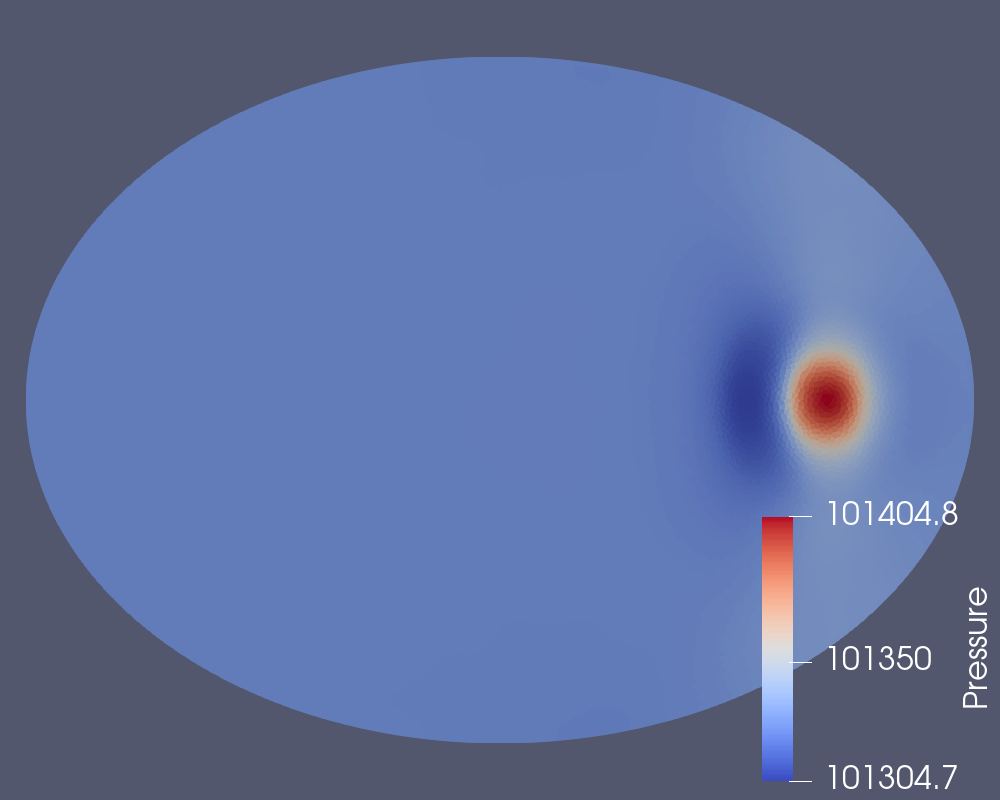
\includegraphics[width=0.47\textwidth]{ellipset01645.png}
}
\caption{Elliptical whispering gallery problem with initial conditions
\eqref{eq:ellipse-initial-conditions}.}
\label{fig:ellipse-simulation}
\end{figure}

\begin{figure}[p]
\centering
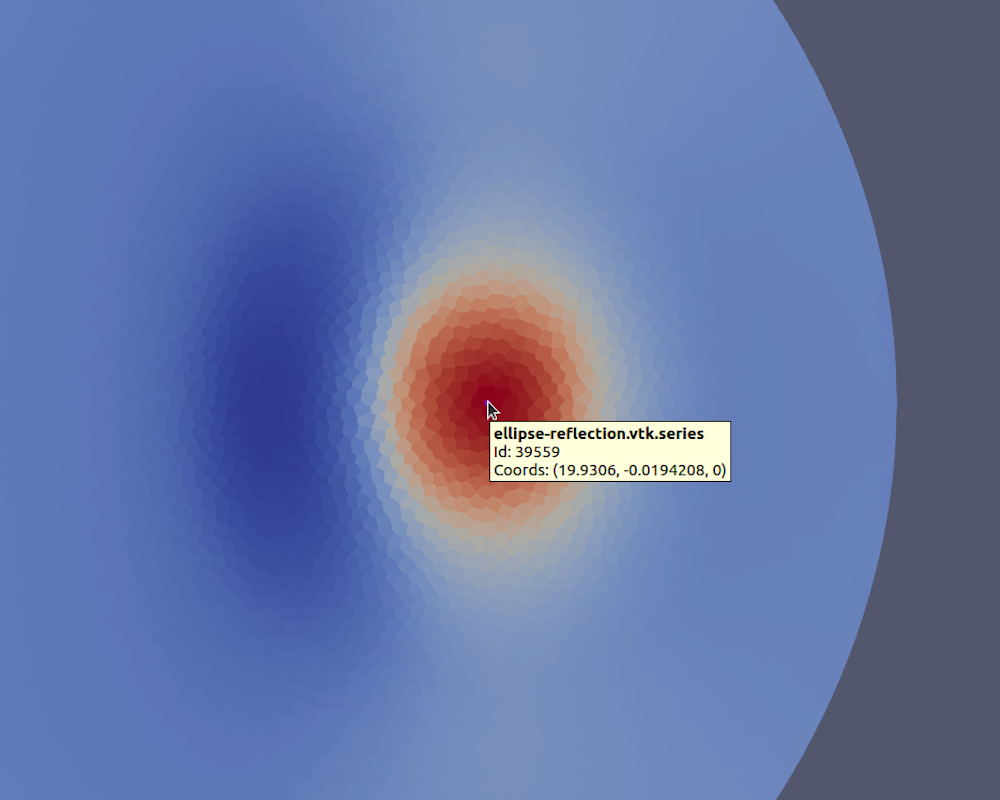
\includegraphics[width=0.65\textwidth]{ellipseF2.png}
\caption{Coordinates of the pressure spike at $t = 0.1645$.}
\label{fig:ellipse-F2}
\end{figure}

\begin{figure}[p]
\centering
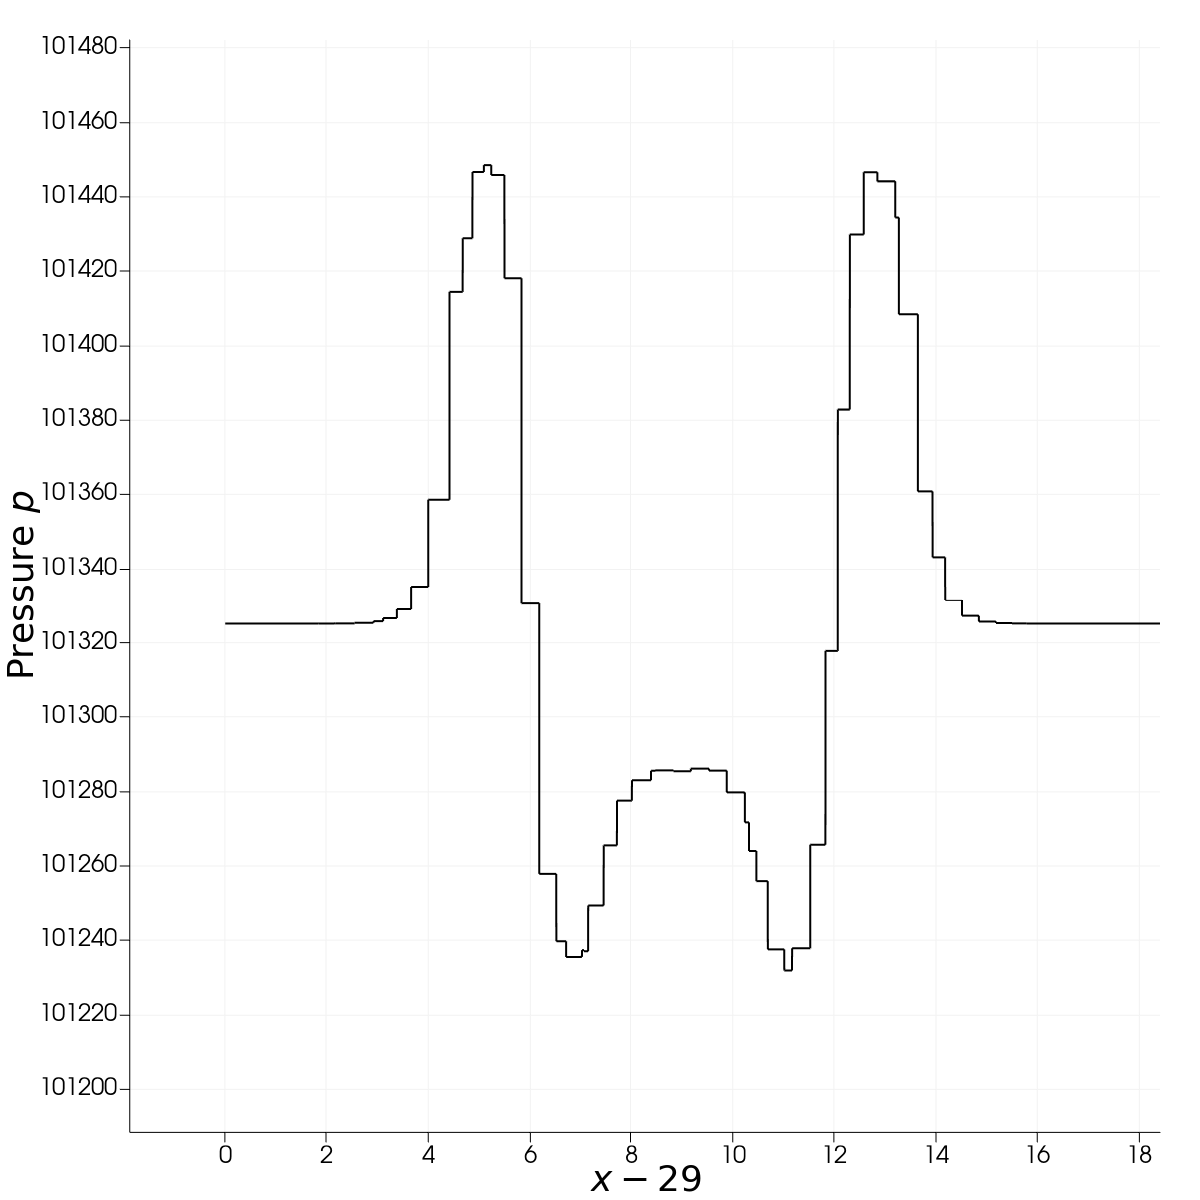
\includegraphics[width=0.85\textwidth]{ellipseP001.png}
\caption{Pressure on the $x$-axis at time $t = 0.01$.}
\label{fig:ellipse-P001}
\end{figure}








































